\chapter{Introduction}

Kaggle is a platform owned by the Kaggle Inc. which is owned by Alphabet Inc. (Google) providing multiple so called challenges in the field of data science, predictive modeling and data analysis. The Kaggle challenge aims at solving so far unsolved tasks or finding a better solution for already solved tasks in a crowdsourcing fashion. Some challenges can be solved for monetary prices, others are hosted for knowledge or training purposes. In order to solve a challenge one must register and submit a solution to the platform to get a score for the submitted solution \cite{kaggle}.

The Google Landmark Recognition Challenge aims at detecting different landmarks in images, such as the Eiffel Tower or the Leaning Tower of Pisa \cite{challenge}.

We chose the Google Landmark Recognition Challenge because we are interested in image processing tasks and the challenge provides a lot of training data. We also wanted to try out Convolutional (Deep) Neural Networks which we previously discussed in the lecture.

The data provided with the challenge contains mainly of two CSV files. The file for training (train.csv) providing the IDs, URLs and Landmark IDs and the file for testing (test.csv) providing IDs and URLs \cite{data}.

Our goal for this part of the project is to prepare the image data and to use different classification methods in order to get good results in detecting landmarks in images.

The evaluation is described in \cite{evaluation}. We need to predict one landmark per image and a corresponding confidence score for it. The overall score will be calculated with the Global Average Precision (GAP) score

\[GAP = \frac{1}{M}\sum_{i=1}^{N}P(i)rel(i)\]

where:\\

\begin{itemize}
	\item $N$ is the total number of predictions returned by the system, across all queries
	\item $M$ is the total number of queries with at least one landmark from the training set visible in it
	\item $P(i)$ is the precision at rank $i$
	\item $rel(i)$ denotes the relevance of prediction $i$: it's 1 if the $i$-th prediction is correct, and 0 otherwise
\end{itemize}

\chapter{Predictive Modeling Steps}
We used opencv-python 3.4.1.15 to extract feature vectors. The procedure is as following: We detect image keypoints, where the number of keypoints is varies depend on image size and color pallet. Than they were sorted based on keypoint response value(bigger is better). The results of this are used to compute a descriptors vectors. Flatten all of them in one big vector generates our feature vector. The descriptors are normalized to a size of 64. If we have less the 32 descriptors then just adding zeros at the end of our feature vector   
Image to feature vector (feature extraction).

\chapter{Training and Test Data}

We chose to create a subset of the original training data for computation time and performance reasons. The original training data has about 1.2 million images which takes too long to process for a one week assignment. We therefore selected the seven most relevant Landmark IDs according to our PCA analysis (IDs: 9633, 6051, 6599, 9779, 2061, 5554, 6651) and chose 2000 images containing those IDs for our training data. The script for downloading this data is attached to this report (download-images.py).

The test data will be chosen accordingly with a size of approximately 25\% of all images.

For reasons of debugging and comparsion we also created a data-set with 200 images. Furthermore we created a data-set with 20000 images to test the performance.  

\chapter{Methods}

Our task in this challenge is to predict whether an image contains a specific landmark or none at all. We had several approaches for such a classification task in the lecture and we chose to use three methods that we discussed previously in class.

\section{KNN}

KNN stands for k-Nearest-Neighbor and describes a typical algorithm that can be used for classification and regression. For classification, the algorithm assigns a data point to a class according to the majority of its k neighbors where k is a pre-defined constant.

\section{SVM}

One very well known method for classification is the Support Vector Machine (SVM) which can be used for a variety of different classification and regression tasks. It usually has a linear output, however, using the so called Kernel Trick allows it to map its inputs into higher dimensional space resulting in non-linear classification of data points.

\section{Logistic Regression}

The Logistic Regression is a special form of regression using the logistic loss as the loss function explained in \cite{logistic-loss}

\[\ell(X, f(X), Y) = \log_2(1 + exp(-Y f(X))).\]

\chapter{Results}\label{results}
First of all the size of our dataset was very challenging. We got a lot of performance and memory problems, so we limited ourself to 2000 images and comparatively simple approaches. For example: We tried to work with a 20000 image set. The feature extraction for this set  took longer than one day and executing knn failed with memory exceptions (8gb RAM was not enough).

The following figure shows the accuracy (in percentage) and time (in seconds) for knn with different ks. 
\begin{figure}[!htb]
	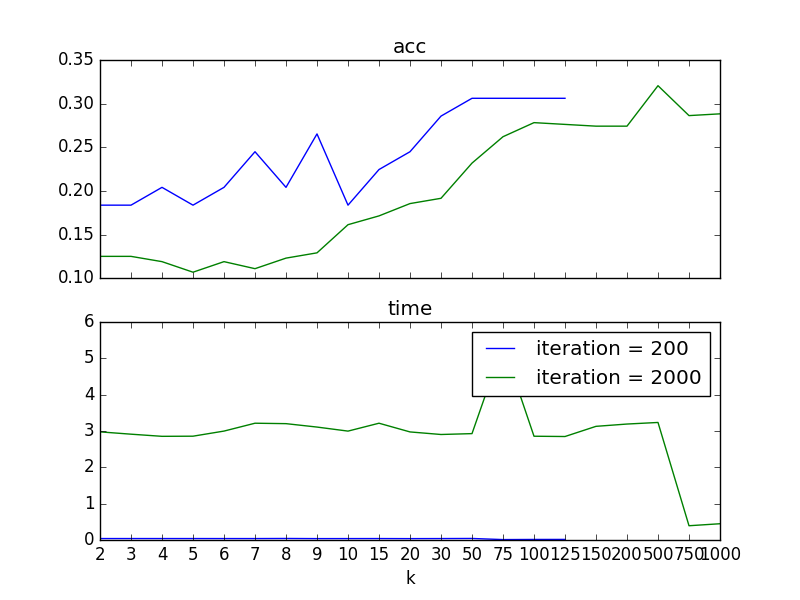
\includegraphics[width=0.85\textwidth]{images/knn}
	\caption{knn for 200 and 2000 images}
\end{figure}
You can see that an increasing k performs better (up to a certain limit). Time usage seems to be not affected by k up to a value of k = 50. 

The second and third figures shows different SVM configurations (kernel, gamma, c). Red and yellow shows $1 - error$, the time is normalized to maximum time usage (0.218 seconds for 200 imgages, 22.318 seconds for 2000 images)
\begin{figure}[!htb]
	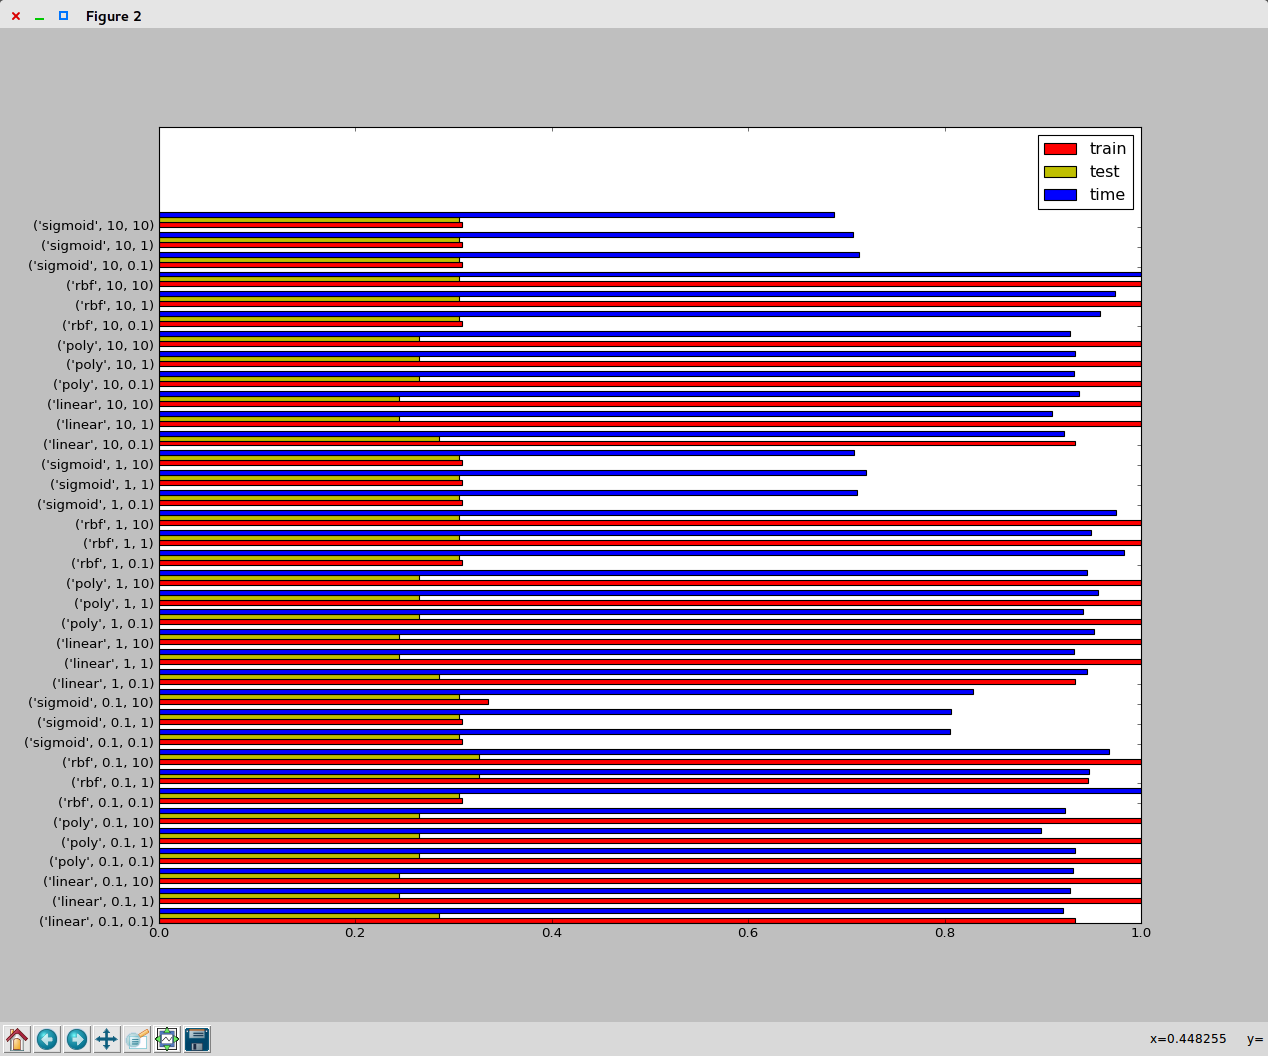
\includegraphics[width=\textwidth]{images/svm200}
	\caption{SVM for 200 images}
\end{figure}

\begin{figure}[!htb]
	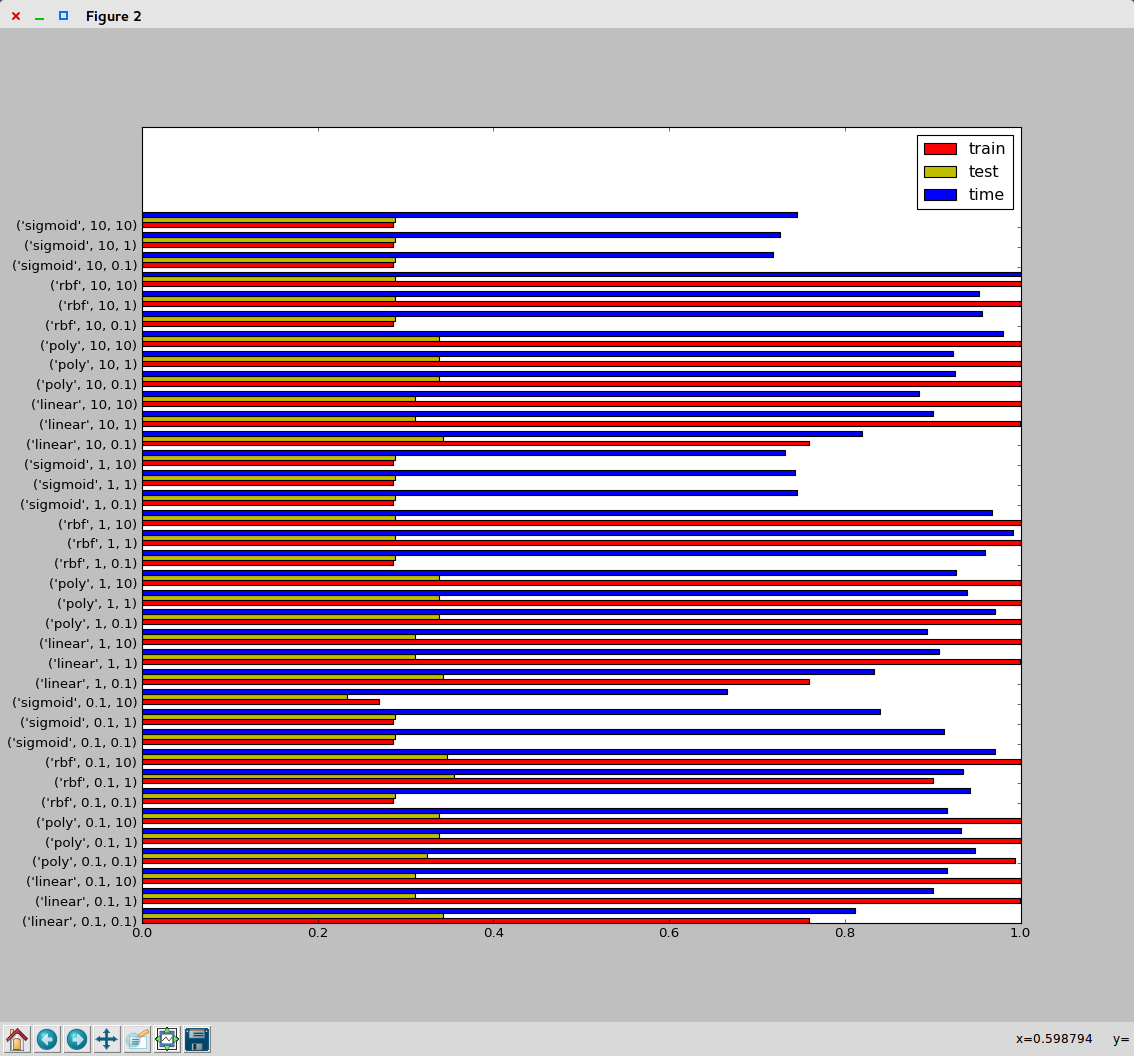
\includegraphics[width=\textwidth]{images/svm2000}
	\caption{SVM for 2000 images}
\end{figure}

Different SVM configurations affects primarily the usage of time. The quality of the model varies by about 5-10\% (1 - test error).\\

\newpage
For Logistic Regression we tested as for SVM different configurations (solver, c). The last two figures show our results.

\begin{figure}[!htb]
	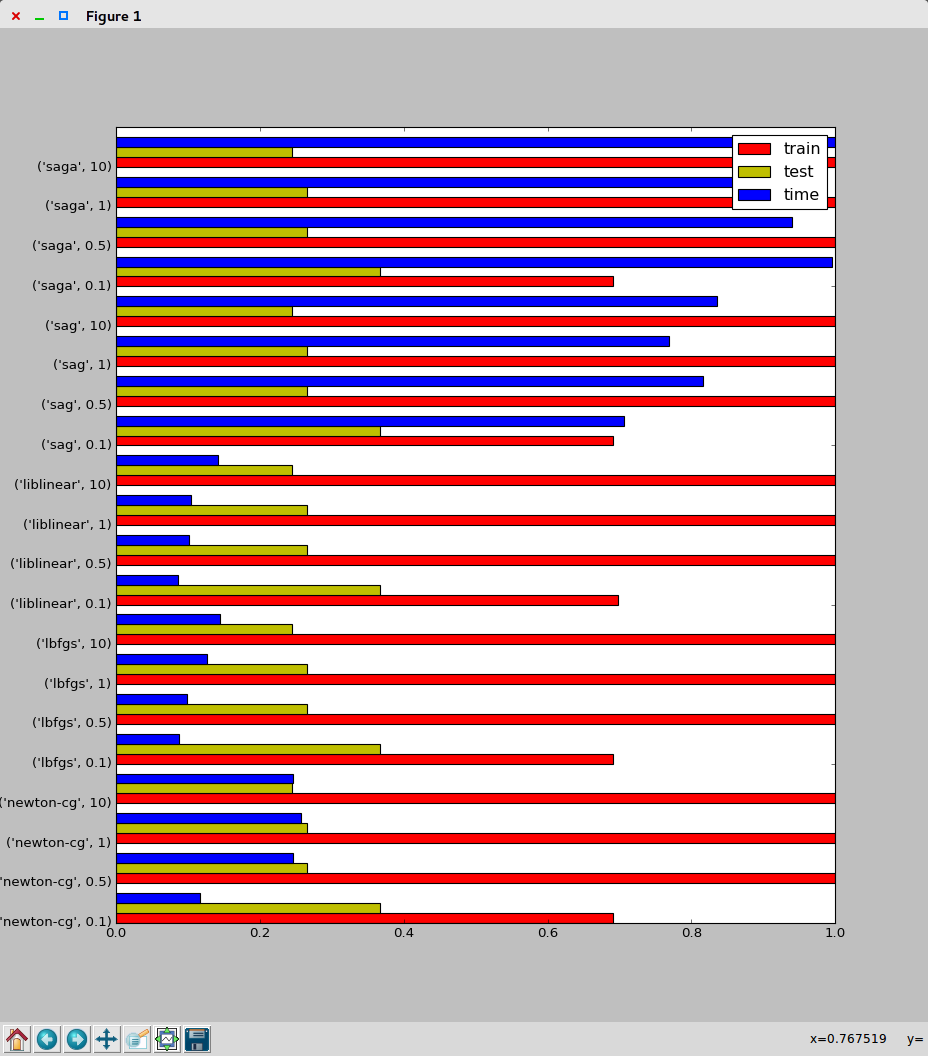
\includegraphics[width=\textwidth]{images/logistic200}
	\caption{Logistic regression for 200 images}
\end{figure}

\begin{figure}[!htb]
	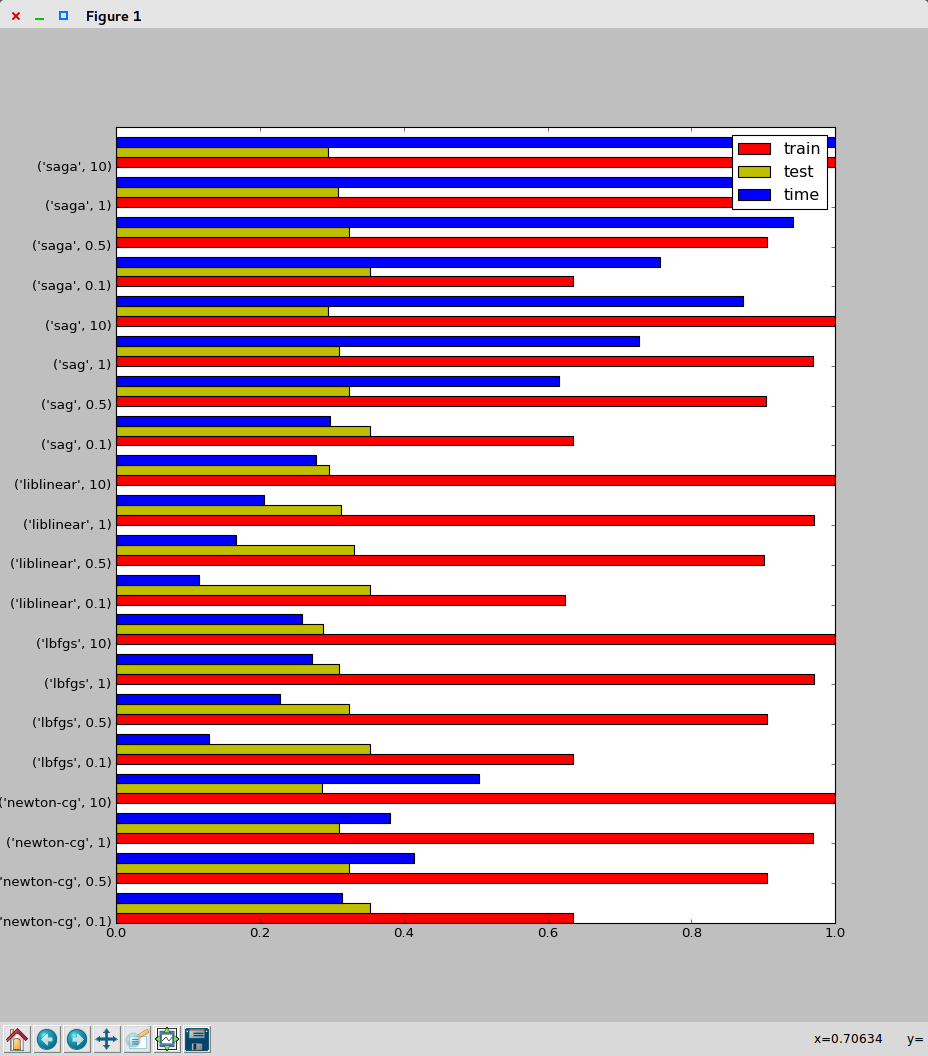
\includegraphics[width=\textwidth]{images/logistic2000}
	\caption{Logistic regression for 2000 images}
\end{figure}

For logistic regression the time is normalized to the maximal time usage (1.543 seconds for 200 images, 16.180 seconds for 2000 images).


\chapter{Method Comparison}

The results shown in chapter \ref{results} show that the accuracy of all approaches are quite bad for 200 or 2000 images. Im most cases there is a small improvement from 200 to 2000 images, so we can hope to achieve further improvements with larger image sets. The problem of these is, that larger sets increase time and memory usage. In all approaches the accuracy varies between 20 and 40\% (random classification, would be 100 percent/ 7 classes = 14\%), most of them nearby 35\%, but the usage of time depends heavily at configuration. Particulary the logistic regression annd the svm approach seems to have solvers/kernels which are unsuitable for our task. The worst configurations need 22 (or 16) while the worst configuration for knn only needs 6 seconds. On the other hand both approaches have configurations which are faster than knn (2-3 seconds time usage). It would be interessting how these configurations would perform with 20000 imgages in comparison to knn.

\chapter{Conclusion}

We introduced three well-known methods for image classification in this project and compared their results for solving the Google Landmark Recognition Challenge.

The results are restricted due to the limitations of RAM. In all approaches there are a prediction precisions near by 35\%. While success seems to be not to depentent from configuration the usage of time is strongly dependent by the configuration.

However, a deep convolutional neural network with a much longer training time is probably the best choice for approaching a task like this.